\documentclass[a4paper]{article}
\usepackage[10pt]{extsizes}
\usepackage[latin1]{inputenc}
\usepackage[T1]{fontenc}
%\usepackage[francais]{babel}
\usepackage[english]{babel}
\usepackage{layout}
%\usepackage{geometry}
%\usepackage{setspace}
%\usepackage{soul}
%\usepackage{ulem}
%\usepackage{eurosym}
%\usepackage{bookman}
%\usepackage{charter}
%\usepackage{newcent}
%\usepackage[super]{nth}
\usepackage{xspace}
\usepackage{textcomp}
\usepackage{lmodern}
\usepackage{appendix} 
\usepackage{comment}
\usepackage{listings}
%\usepackage[inline]{asymptote}
\usepackage{graphicx}
\usepackage{wrapfig}
\usepackage{caption}
\usepackage{subcaption}
\usepackage[outdir=./data/]{epstopdf}
\usepackage{svg}
\usepackage{placeins}
%\usepackage{MyMnSymbol}
%\usepackage{mathpazo}
%\usepackage{mathptmx}
%\usepackage{url}
%\usepackage{comment}
%\usepackage{moreverb } 
%\usepackage{listings}
%\usepackage{fancyhdr}
\usepackage{color}
%\usepackage{colortbl}
\usepackage{mathtools,amssymb,amsfonts,amsthm}
\usepackage[squaren, Gray, cdot]{SIunits}
%\usepackage{mathabx}
\usepackage{cancel}
%\usepackage{mathrsfs}
%\usepackage{asmthm}
%\usepackage{makeidx}
\usepackage{parskip}
\newcommand\nth{\textsuperscript{th}\xspace}
%\setlength{\textwidth}{410pt}
%\setlength{\oddsidemargin}{25pt}
%\allowdisplaybreaks
\title{Above-Threshold Ionization in the Strong Field and Long-Wavelength Tunneling Limit}
\author{Yann Gouttenoire}
\date{May-July 2015}

\setlength{\oddsidemargin}{0pt}
\setlength{\marginparsep}{0pt}
\setlength{\textwidth}{454pt}
%\linespread{0.5}
\lstset
{
breaklines=true,
basicstyle=\footnotesize,
frame=single,
columns=fullflexible,
literate={*}{{\char42}}1
         {-}{{\char45}}1
}

\newcommand{\shiftright}[2]{\makebox[#1][r]{\makebox[0pt][l]{#2}}}
\newcommand{\shiftleft}[2]{\makebox[0pt][r]{\makebox[#1][l]{#2}}}

\renewcommand\thesubfigure{\roman{subfigure}}

\begin{document}
\begin{comment}
\end{comment}

\makeatletter

  \begin{titlepage}
  \centering
  {\LARGE \textbf{Above-Threshold Ionization in the Strong Field and Long-Wavelength Tunneling Limit}} \\
      \vspace{1cm}
  {\large \@author} \\
      \vspace{1cm}
  {\textbf{Master 1 and 2$^{\textbf{nd}}$ year at Magist\`ere de Physique Fondamentale d'Orsay}} \\
      \vspace{1cm}
      \begin{figure}[h]
      \centering
    
\includegraphics[width=0.30\textwidth]{logo/magistere.jpg}
      \end{figure}
  {\textbf{which is a certificate delivered by University Paris-Sud, member of University Paris-Saclay}} \\ 
        
   \begin{figure}[h]
   \centering
   \begin{subfigure}[l]{0.30\textwidth}
       
\includegraphics[width=\textwidth]{logo/upsud}
   \end{subfigure}
   \hfill
   \begin{subfigure}[r]{0.30\textwidth}
       
\includegraphics[width=\textwidth]{logo/upsaclay}
   \end{subfigure}
   \end{figure}
        \vfill

 {\LARGE \textbf{Internship supervisors:}}\\
       \vspace{0.5cm} 
  {\large \textbf{Eric Charron$^{1}$ and Misha Ivanov$^{2}$}} \\
       \vspace{0.5cm}
  {\large \textit{$^{1}$Institut de Chimie Mol\'eculaire d'Orsay, Orsay, France}} \\   
  {\large \textit{$^{2}$Max Born Institute, Berlin, Germany}} \\
   \begin{figure}[h]
   \centering
   \begin{subfigure}[l]{0.3\textwidth}
       
\includegraphics[width=\textwidth]{logo/ismo}
   \end{subfigure}
   \hfill
   \begin{subfigure}[r]{0.3\textwidth}
       
\includegraphics[width=\textwidth]{logo/mbi}
   \end{subfigure}
   \end{figure}
      \vspace{-0.2cm}
  {\large\textbf{	\@date}} \\
      \vfill
   
 
        \end{titlepage}
\makeatother

\newpage
\unboldmath{\tableofcontents}
\newpage


\section{Introduction}

In the early 1960s, in California, a physicist named Theodore H. Maiman invented the first source of light based on the mecanism of amplification by way of stimulated emission: the Q switched Ruby laser. This would not have been possible without the invention of optical pumping methods by the french physicists Alfred Kastler and Jean Brossel in the early 1950s. Then the laser was born and its most important particularity is to emit light coherently which leads to an electromagnetic wave with a very narrow spectrum.
Then, the spectacular advances in laser source, covering a range of frequencies from micro waves to far ultraviolet have offered new opportunities for exploring the structure and the dynamic of atoms and molecules, controlling their internal and external degrees of freedom, and for generating new types of radiation. 
\par
The possibility to push laser intensity to order of magnitude beyond the atomic field acting on the outer shell electrons - a possibility which relies on the development of short laser pulse - has opened the way to the investigation of multiphoton processes. These processes can reveal a host of aspects different from those accessible to the well established one-photon transitions, with their restricted selection rules.
The most important are the above-threshold ionization and the high-harmonic generation.
\par
During the 1970's, experiments were absolute measurements of the dependance of the ionization yield on the lazer intensity.
It was a great advance when in 1979, Agostini \textit{et al} (see \cite{Agostini_1979}) measured the energy of the ionized electrons which are ejected after the illumination of atoms with a laser pulse. This is the now well-known photo-electrons spectrum (PES). It was a surprise when they observed that the electrons could absorb many more photons than the minimum number required to be promoted to the continuum. This process called above-threshold tonization (ATI) revealed new channels of ionization.
The second phenomenon of main interest, the high-harmonic generation is first observed up to very high order by L'huillier \textit{et al} in 1989 (see \cite{Li_1989}). This can be explained by the recollisional model: half an optical cycle after ionization, the electric field will change direction, and the electron will be accelerated back toward the ionic core with which it can recombine by emitting a single high energy photon. 
\par
More recently, in 2009, Blagua \textit{et al} (see \cite{Blaga_2009} and \cite{Quan_2009}) observed low-energy structures (LES) in the photo-electrons spectrum. In 2012, K\"astner \textit{et al} (see \cite{Kastner_2012_soft}) revealed that the soft recollisions where the electron rescatters with the parent nucleus with a large impact parameter are at the origin of the presence of these peaks at low energy.
\par
During this 3 months internship, I have spent the most of the time implementing a code which computes the so-called above-threshold ionization spectrum (photo-electrons spectrum). The simulation is based on the Monte-Carlo method: we compute classic trajectories of an electron just after the ionization step, its positions and velocities at ionization time resulting from the theory of tunneling ionization. 
On the one hand, with a view to making sure that the code was correct, I tried to reproduce some results in two differents papers when using the same parameters. First, I tried to compute the photo-electrons spectrum and to plot some interesting trajectories published in the article \cite{Hu_1997}. Second, I tried to plot the low-energy spectrum published in the article \cite{Kastner_2012_pulse}.
On the second hand, I replaced the hydrogenoid atom by a chiral molecule and the linear polarization of the laser field by a circular one and I tried to look for a signature of the chirality in the LES.


\section{Mecanisms of ionization induced by a Strong field}
Let's us first defined some quantities used in this report. $F$ is the electric field defined as
\begin{equation}
\label{electric_field}
F=F_{0} f(t)\cos{\omega t} \mathbf{e_{z}} + \beta F_{0} f(t)\sin{\omega t} \mathbf{e_{x}}
\end{equation}
where the envelop of the pulse laser f(t) is such that
\begin{equation}
\label{envelop}
 \lim_{t\to\pm\infty} f(t)=0.
\end{equation}
$I_{p}$ is the ionization potential of the atom or molecule considered. $U_{p}$ is the kinetic energy of the free electron in the electric field averaged over one period of the field. It is called \textit{ponderomotive energy} or \textit{quiver energy} and is given by:
\begin{equation}
U_{p}=\left< \frac{1}{2}m \left(\frac{eF}{\omega}\sin{\omega t} \right)^{2} \right>_{T} = m \left( \frac{eF}{2\omega} \right)^{2} \; [SI] \; = \frac{F^{2}}{4\omega^{2}} \; [\text{au}],
\end{equation}  
where $F$ and $\omega$ are the amplitude and the pulsation of the electric field.

It is a common practice in the atomic, molecular, and optical fields to use atomic units defined by $m_{e}=1$, $e=1$ and $\hbar=1$. The energy is also often exprimed in eV or in unit of $U_{p}$. Here are some useful conversions
\begin{align*}
\text{intensity: } 1 \text{ au } & = 3.5094451\times10^{16} \text{ W/cm$^{2}$ }  &\text{energy: } 1 \text{ au }&= 27.211608 \text{ eV} \\
\text{Up: } 1\text{ [eV]} &= 0.09337 \text{ [W/cm$^{2}$] }\lambda^{2}\text{ [m] } &\text{time: } 1 \text{ au }&=24.1888421\times10^{-18} \text{ s} 
\end{align*}

For information, the electric fields used for ionization are essentially laser pulses with pulse durations from nanosecond to femtosecond and wavelenghts from infrared to visible.
The strength of the field called intensity is the flux of the electric energy transmitted through an imaginary surface. It can vary from $10^{12}$ W/cm$^{2}$ to $10^{16}$ W/cm$^{2}$.
 

\subsection{Two ionization regimes: tunneling ionization and multiphoton ionization}
Even with the first laser, the Q switched Ruby, the radiation was intense enough to make observable air breakdown and a bunch of theoretical physicists started to show a strong interest for the ionization phenomenon. In his famous paper, published in 1965, Keldysh showed that during the ionization, two regimes are in competition. In weak fields, electrons are promoted into the continuum by the simultaneous absorption of enough photons \textbf{(see figure)}. This process called multiphoton ionization (MPI) is observed for the first time the same year by Voronov and Delone (see \cite{Voronov_1966}). However, when the laser intensity increases, at large distances from the atoms, the Coulomb potential is overwhelmed by the instantaneous laser field, producing a barrier through which an electron can escape via quantum tunnelling (see figure (\ref{tunneling_ionization})). That process called tunnel ionization or quasistatic MPI was not immediately accepted as being valid physically until it was observed for the first time in 1985 by Chin \textit{et al} (see \cite{Chin_1985}). The transition between this two regimes of ionization is defined by the so-called \textit{adiabatic parameter} $\gamma$ defined by
\begin{equation}
\gamma=\sqrt{\frac{I_{p}}{2U_{p}}} = \sqrt{\omega\frac{\sqrt{2I_{p}}}{F}}.
\end{equation}
The weak field and high-frequency limit ($\gamma \gg 1$) corresponds to the MPI regime whereas the tunneling regime is attributed to the strong field and low-frequency limit ($\gamma \ll 1$). In the tunneling regime, we can give a clear meaning of $\gamma$, it is the product of the tunneling time $\tau_{T}$ and the frequency of the field $\omega$ (see \cite{Misha_2014}). Therefore, in the tunneling limit, $\tau_{T} \ll \frac{1}{\omega}$, the field oscillates slowly enough to let the electron tunneling through the barrier. 

The tardive observation of the tunnel ionization was due to the impossibility to make pulse laser short enough. Indeed, for a long pulse laser, we can not neglect the MPI contribution which becomes significant during the rising and falling part of the pulse where the laser intensity is weaker and then $\gamma \gg 1$ (see \cite{Chin_2004}).
\par 
During this internship, I studied ionization processes in the long-wavelengh limit (few $\mu$m). One of the main reasons is that this allow a total classical description of the electron after it tunnels out. The next section introduces the tunnneling rate for a given field value and a given final velocity for the electron.

\subsubsection{The tunneling rate}

The probability of tunneling ionization of a hydrogen atom in an electrostatic field was first determined by Landau and Lifshitz in 1965 (see \cite{Landau_1965}) and is given by $w(0)=(4/F)\exp(-2/3F)$. In 1966 the scope of the above formula was extended by Perelomov, Popov, Terent\'ev (PPT) for an arbitrary state of the hydrogen atom (see \cite{PPT_1966}). Then, in 1986 Ammosov, Delone and Krainov (ADK) derived the quasi-classical tunneling limit of the equation of PPT (see \cite{ADK_1986}). Finally, in 1991 the ADK formula is extended in order to take into account the distribution of electron velocities after tunneling (see Delone and Krainov \cite{Delone_1991})
\begin{equation} 
\label{ADK_distribution}
w(\phi_{i},v_{\perp i})=w(0)w(1), \quad w(0)=\frac{4}{F}\exp(-\frac{2}{3}\frac{[2I_{p}]^{3/2}}{F}), \quad w(1)=\frac{1}{\pi F}\exp(-\frac{\sqrt{2I_{p}}v_{\perp}^{2}}{F}),
\end{equation}
where the index $i$ denotes the quantities at the time of ionization and where $1/\pi F$ derived from the condition of normalization over the perpendicular velocity. 
The velocity parallel to the laser polarisation has been took equal to 0 (see \cite{Hu_1997}). We insist that the above expression is only valable in the tunneling regime.
\par
This ionization rate formula has been used to weight classical trajectories in my simulations. For each trajectory, I picked the phase of the electric field at birth $\phi_{i}$ as well as each component of the perpendicular velocity at birth $v_{\perp X i}$, $v_{\perp Y i}$ where (X,Y) denotes the polarization plane. Then, I computed the probability for having such initial conditions for both the field and the electron velocity with the above formula.
\par
However, when the field is linearly polarized, the system is cylindrical symmetric by reference to the laser polarization and we would prefer picking only the radial component $v_{\perp i}=\sqrt{v_{\perp X i}^{2} + v_{\perp Y i}^{2}}$ instead of the two components $v_{\perp X i}$ and $v_{\perp Y i}$. Then, we have to take into account the additional Jacobian factor $v_{\perp}$ which appears when we transform cartesian coordinates into cylindrical coordinates,
\begin{equation}
w(\phi_{i},v_{\perp i})=w(0)\bar w(1), \quad w(0)=\frac{4}{F}\exp(-\frac{2}{3}\frac{[2I_{p}]^{3/2}}{F}), \quad \bar w(1)=\frac{v_{\perp}}{\pi F}\exp(-\frac{\sqrt{2I_{p}}v_{\perp}^{2}}{F}).
\end{equation}
In the papers mentionned previously, the ionization rate is obtained by solving the time-dependent Shr\"odinger equation and by doing approximations. The main approximation in the so-called Strong Field Approximation (see \cite{Misha_2014}). This leads to the derivation of the transition amplitude between the ground state and the final state where we completely neglect the Coulomb potential in the continuuum. The final state is then simply the wave function of a free electron in an electric field and is called \textit{Volkov} state. One of the motivation for a such approximation is that the the Volkov wave function has an analytic expression.
\par
Since the early 1990, the strong field physics in the tunneling regime has attracted a considerable attention. An important reason for such a thing, is that $\gamma \ll 1$ which is similar to $U_{p} \gg I_{p}$ is compatible with the quasi-classical limit defined by $U_{p} \gg \omega$. This is the case for mid-infrared laser fields where the wavelenght is $\lambda \propto 2\,\micro\text{m}$. Upon this condition, we can consider the electron in the continuum as following classical trajectories. Quantum effects like the spreading of the wave function in phase space are encoded in the factor $w(1)$ in the ionization distibution (\ref{ADK_distribution}). It is quite suprising that such quantum effects which occur during the propagation of the wave function in the vacuum can be conceal in the distribution of initial velocities. The quantum properties are then propagated as the electron accomplished its classical trajectory. 
\par
Besides, in contrast to the MPI, in the tunneling limit the position of the electron in the continuum is really clear.
Indeed, the position of the electron $x_{i}$ when tunneling out of the barrier can be derived following a 1 dimensional and classical model (see figure (\ref{tunneling_ionization})). $x_{i}$ is solution of the equation of energy conservation between the time the electron tunnels in and the time the electron tunnels out when supposing the electron is at rest for both instants.
\begin{equation}
-\frac{1}{| x_{i} |}+x_{i}F_{i}=-I_{p} \Rightarrow Fx^{2}+I_{p}x-1=0 \Rightarrow x_{i\pm}=-\frac{I_{p}}{2F_{i}}\pm\frac{\sqrt{I_{p}^{2}-4F_{i}}}{2F_{i}}
\end{equation} 
where $x_{i+}$ and $x_{i-}$ are repectively the positions of the electron when tunneling in and when tunneling out.

\begin{figure}[h] 
\centering
%\def\svgwidth{<desired width>}
 \input{data/tunnel.pdf_tex}
 \caption{Quasistatic picture of tunneling ionization}
 \label{tunneling_ionization} 
\end{figure}

\section{Classical pictures}

In the previous section, we explained that the character of the dynamic of strong field atomic ionization depends on the value of the adiabatic parameter $\gamma \propto \sqrt{\frac{\omega}{F}}$. When the latter is weak, that is in the strong field and low-frequency limit also called the tunneling limit, we can describe the ionized electron (or photo-electron) in the continuum classically. Therefore, the position and velocity of the electron interacting with both the Coulomb potential of the parent ion and with a linear polarized laser field along $x$ can be derived from the Newton equation
\begin{equation}
\frac{d \mathbf{v(t)}}{dt}=-\frac{\mathbf{r(t)}}{r(t)^{3}}-F\mathbf{e_{x}}\cos(\omega t) f(t) 
\end{equation}
Let's try a first approach in which we neglect the Coulomb field, following the example of the Strong Field Approximation mentionned previously. We also consider that the electron after tunneling out at the time $t_{i}$ is at rest. Then, its velocity at a time $t>t_{i}$ follows
\begin{align}
\label{velocity_free_motion}
v_{x}(t)&=-\frac{F}{\omega}\left[\sin(\omega t) f(t)-\sin(\omega t_{i}) f(t_{i})\right] \\
v_{\perp}(t)&=0
\end{align}
We immediately noticed that the velocity along the field is the superposition of two contributions. The first is the velocity associated with the oscillatory motion, also called \textit{quiver} motion. The second is the velocity related to the translational motion, also called the drift motion. Because of the condition (\ref{envelop}), the drift velocity is the one that we measure in experiment when the field is switched off. It depends only on the phase value of the field at the time $t_{i}$ when the electron becomes free. This sensitivity of the photo-electron energy to the time of ionization is demonstrated by Gallaguer in 1988 who managed to control $t_{i}$ by varying the ionization potential of the atom. For this purpose, he used Rydberg atoms excited to specific states (see \cite{Gallagher_1988}).
\par
Then, we integrate the above formula and derive the position $x$ of the free electron along the field
\begin{equation}
\label{position_free_motion}
x(t)=\frac{F}{\omega}\left[\cos(\omega t)-\cos(\omega t_{i})+\sin(\omega t_{i})\omega(t-t_{i})\right] \\
\end{equation}
where we neglected the position of the electron after tunneling as well as the fall of the envelop.
The above equation tells us that the electron has two possibilities: it can either escape or be driven back and recollide with the parent ion. The condition of rescattering with the ionic core at a time $t_{c}$ is the condition of zero displacement between the time of ionization $t_{i}$ and the time of collision $t_{c}$
\begin{equation}
\label{zero_displacement}
x(t_{c})=0 
\end{equation}
The resolution of this equation shows that the electron rescatters only for ionization after the maximum of the peak, that is for $\omega t_{i} \in [0^{\circ},90^{\circ}]$. Otherwise, for $\omega t_{i} \in [-90^{\circ},0^{\circ}]$ the electron never comes back in the vicinity of the nucleus. The difference between these two cases is pure effects of the drift component of the velocity $v_{drift}=\frac{F}{\omega}\sin{\omega t_{i}}$. After the peak  of the field $v_{drift}$ is positive and drives the electron back but before the peak $v_{drift}$ is negative and pushes the electron away. \\
Furthermore, the electron can rescatter several times. The numerical resolution of the zero displacement condition (\ref{zero_displacement}) shows that the electron comes back exactly one time for $\omega t_{i} \in [12.55^{\circ},90^{\circ}]$, 3 times for $\omega t_{i} \in [7.37^{\circ},12.55^{\circ}]$, 5 times for $\omega t_{i} \in [5.24^{\circ},7.37^{\circ}]$ and so on. Asymptotically, the electron comes back an infinite numbers of times when $\omega t_{i}$ tends to the peaks of the field. The figure (\ref{successive_recollision}) shows the graphical resolution of equation (\ref{zero_displacement}) in the case of one and three recollisions.
\begin{figure}
\centering
%\def\svgwidth{<desired width>}
 \input{data/zero_displacement.pdf_tex}
 \caption{Successive recollisions of the electron with the parent ion in the classical model. On the left figure, $\omega t_{i}$ is contained in $[12.55^{\circ},90^{\circ}]$ and the electron recollides only one time. On the right figure, $\omega t_{i}$ is contained in $[7.37^{\circ},12.55^{\circ}]$ and the electron recollides exactly three times.}
 \label{successive_recollision} 
\end{figure}
\par 
When the electron rescatters, it has few possibilities:
\begin{itemize}
\item
first, it can recombine with the parent ion and use its kinetic energy for emitting light, it is the so-called high harmonic generation (HHG),
\item
second, it can rescatter inelastically and use its kinetic energy for ionizing a second electron, it is the so-called sequential ionization,
\item
finally, it can scatter "elastically" (we will understand the quotation marks later), this leads to the so-called above-threshold ionization (ATI).
\end{itemize}
The classical picture of ionization we just discussed is also known as the \textit{simple-man model} or \textit{three-step model}:
the strong field removes the electron, accelerates it and drives it back to recollide with the ionic core.
In the next part, we will discuss how this naive description can predict the basic features of the high harmonic and above-threshold spectra.

\section{High Harmonic Generation}

When we measure the electromagnetic response emitted from a dilute gas irradiated by a strong laser field, we observe a serie of peaks separated in energy by the photon energy of the laser field. (FIGURE) The shape of the spectrum shows a rapid decline at low energy, followed by a plateau of relatively constant harmonic intensity and then a sharp cut-off at high energy.
In 1992, Krause \textit{et al} (see \cite{Krause_1992}) investigated the evolution of the energy of the maximum observable harmonic with the laser intensity, the wavelengh and the ionization potential of the outershell electron. Thus, they derived the well-known cut-off law
\begin{equation}
\label{cut-off}
E_{max}=I_{p}+3U_{p}.
\end{equation}
In 1993, Corkum (see \cite{Corkum_1993}) showed that $3U_{p}$ corresponds to the maximum kinetic energy of the electron at the time of the recollision with the parent ion. This kinetic energy has been gained when the electron was accelerating in the laser field by absorbing n photons. Then the energy of the unique photon emitted during the recombination process is an integer multiple $n\omega$ of the laser frequency. This explains why the spectrum of the electromagnetic response is only constituted of harmonic of the strong laser field. This explains also its name: high harmonic spectrum.
\par 
Let's now use the three-step model described previously in order to explained the cut-off law (\ref{cut-off}).
With the expression of the velocity of the electron in (\ref{velocity_free_motion}) as well as the condition of zero-displacement in (\ref{zero_displacement}), we can deduct the kinetic energy $E_{k}$ of the electron at the time of the recollision $t_{c}$
\begin{equation}
E_{k}(t_{c})=2U_{p}\left[ \sin{\omega t_{c}}-\sin{\omega t_{i}}\right ]^{2}
\end{equation}
where we neglected the falling contribution of the envelop ($f(t)=f(t_{i})=1$). \\
On the figure (\ref{successive_recollision}), we can see that for a given phase of ionization $\omega t_{i}$, the electron can rescatter several times with the ion and then, it corresponds several values of the kinetic energy $E_{k}$. 
The left side of figure (\ref{kinetic_energy}) shows the kinetic energy $E_{k}$ at the time of the first recollision plotted as a function of the phase of ionization $\omega t_{i}$. The maximum value of $E_{k}$ is $3.17U_{p}$ and the cut-off law (\ref{cut-off}) is clarified. It is attained for $\omega t_{i}=18.0^{\circ}$ and $\omega t_{c}=252.0^{\circ}$. \\
\begin{figure}
\centering
 \input{data/simpleman.pdf_tex}
 \caption{Kinetic energy of the electron at the time of the first recollision as a function of the phase of ionization (on the left) and detected kinetic energy of the electron after having been back-scattered (on the right)}
 \label{kinetic_energy} 
\end{figure}

HHG has attracted a considerable attention in connection to the possibility to generate attosecond pulses (see \cite{Ivanov_2009}).
Then it becomes possible to study processes that occur on time scales approaching the atomic unit of time ($\sim 24\,as$), like electrons dynamic in atoms and molecules. 
Attosecond pulses can be used in pump-probe scenario, where the first pump laser pulse prepares the system by initiating the dynamic of interest. Then the second laser pulse investigates the evolved dynamic. By varying the time delay between the two pulses, we can make a time-delayed imaging of the evolution of the system.


\section{Above-Threshold Ionization}

When we measure the kinetic energy of the photo-electrons ejected from a dilute gas illuminated by a strong laser field, we obtained a serie of peaks separated in energy by the photon energy of the laser field. (FIGURE) The spectrum exhibits at low energy ($[0,2U_{p}]$) an abrupt decreasing slope followed by a plateau ($[2U_{p},8U_{p}]$) and again an abrupt decreasing slope which can reach $10 U_{p}$. This reminds us the harmonic spectrum obtained by mesuring the electromagnetic responsed. However, the energy of the cut-off which were $3U_{p}$ in the harmonic spectrum, extends now to $10U_{p}$. This amazed the physicist in the early 1990 because this means that the electron absorbs many more photons that the minimum required for being promoted in the continuum and that a new channel of photon absorption is opened. It was well-known that a bounded electron could absorb photons but it was not easy to accept that even an electron in the continuum could absorb photons. That is why the photo-electron spectrum was called the above-threshold ionization spectrum (ATI spectrum).
\par
The low energy region of the spectrum, up to two $U_{p}$, is simply the energy due to the drift component. Indeed, with the expression (\ref{velocity_free_motion}) of the velocity of the electron as well as the condition (\ref{envelop}), we can derive the expression of the kinetic energy detected when the laser field is switched off
\begin{equation}
E_{k}^{\infty}=2U_{p}\sin(\omega t_{i})f(t_{i}) \quad < \quad 2U_{p}
\end{equation}
The sharp decrease at low energy can be explained by the fact that due to the tunneling rate (factor $w(0)$ in (\ref{ADK_distribution})), they are more electrons ionized when the electric field is at its maximum, and this corresponds to a minimum of $\sin(\omega t_{i})f(t_{i})$ in the above expression.
\par
However, the high energy region is intriging because it is well-known that a free electron can not absorb photons. This stems from the conservation of the energy and momentum. Let's consider a collision between an free electron with momentum $\mathbf{p_{i}}$ and a photon with momentum $\mathbf{k_{i}}$ followed by the absorption of the photon by the electron. We denote $\mathbf{p_{f}}$ the final momentum of the electron. The energy-momentum four-vector of the system \{electron$+$photon\} is given by
\begin{equation}
\left(
\begin{array}{c}
E_{tot}\\
\mathbf{p_{tot}}\\
\end{array}
\right)
=
\left(
\begin{array}{c}
E_{e}^{i}\\
\mathbf{p_{i}}\\
\end{array}
\right)_{e^{-}}
+\left(
\begin{array}{c}
E_{\gamma}\\
\mathbf{k_{i}}\\
\end{array}
\right)_{\gamma}
\end{equation}
where $E_{e}=\sqrt{(pc)^{2}+(mc^{2})^{2}}$ and $E_{\gamma}=\hbar kc$.
The conservation of the energy and momentum is given by
\begin{align}
\label{momentum_conservation}
\mathbf{p_{f}}&=\mathbf{p_{i}}+\hbar \mathbf{k_{i}}, \\
\label{energy_conservation}
E_{e}^{f}&=E_{e}^{i}+E_{\gamma}.
\end{align}
Then, if we note $\theta$ the angle between $\mathbf{p_{i}}$ and $\mathbf{k_{i}}$, we obtain
\begin{align}
E_{e}^{f2}&=E_{e}^{i2}+E_{\gamma}^{2}+2\sqrt{E_{e}^{i2}-(mc^{2})^{2}}E_{\gamma}\cos{\theta}, \\
E_{e}^{f2}&=E_{e}^{i2}+E_{\gamma}^{2}+2 E_{e}^{i}E_{\gamma}.
\end{align}
If we now take the difference between these two equations, we get
\begin{equation}
E_{e}^{i}=\sqrt{E_{e}^{i2}-(mc^{2})^{2}}\cos{\theta} \quad \Rightarrow \quad E_{e}^{i2} \tan^{2}{\theta} = -(mc^{2})^{2}
\end{equation}
which can not be satisfied for a particule of finite mass $m\neq0$ like it is of course the case of the electron. Thus, we just demonstrated that a free electron can not absorb photons.\footnote{However, for really strong field such that $U_{p}$ is becoming comparable with the electron's rest energy $mc^{2}$, we enter in the relativistic regime and we can not neglect the Lorentz magnetic force anymore. The latter opens a new channel of multi-photons absorption}
This can also be understood classically: in an electric field, the acceleration of the electron will exacty be balanced by the decceleration counterpart when the field will change its direction.
\par
Finally, the only component which remains after the pulse is the initial offset, constant over time, which is responsible for the translational motion. We have to search for a mecanism which increase this drift energy up to $10 U_{p}$.
In experiment, when the laser pulse is long enough, the photo-electron can leave the focus of the laser beam before the latter is swithed off. Therefore the electron will pass through region of space where the electric field is inhomogeneous and will undergoe a force which drives the electron in the region of weak field. Indeed, the electric field at one turning point of the harmonic motion can exceed the electric field at the other one. Finally, the drift velocity in the opposite direction of the gradient of the field is increased. However, this mecanism disappears for ultrashort laser pulse and then, it can not explained the high energy region of the ATI spectrum.
\par
In fact we can not build a predictive model for the ATI spectrum if we consider the electron as free and if we neglect the interaction of the electron with the Coulomb potential of the parent ion. When the electron is driven back and recollide with the parent ion, the coulomb attraction becomes sufficiently intense to dephased the harmonic motion. Then, a transfer of energy between the oscillatory motion and the drift motion occurs. When coupled with the Coulomb field, the electric field behaves like a reservoir of energy for the electron. This underlying mecanism which explained the multiphoton ionization far from the threshold has been intuited by Kuchiev in 1987 (see \cite{Kuchiev_1987}) when he explained that "the electron in this process plays the role of an absorber of field energy, the role of antenna". 
\par
But the absorption of many photons during electron-ion collisions were already well-known by plasma physicist as free-free transitions or inverse bremstrahlung. They were considered as the mecanism responsible for the electron avalanche in laser-induced air breakdown (see \cite{Chin_2004}).
\par
As for the harmonic spectrum, the position of the cut-off in the ATI spectrum can be predicted with a classical three-step model. This was predated in 1994 by Paulus \textit{et al} (see \cite{Paulus_1994}). We suppose a field linearly polarized (along x) such that the trajectory of the electron evolves in a plane (xy). The velocity of the electron just before the recollision is the expression (\ref{velocity_free_motion}) evaluated at the time $t_{c}-\epsilon$ where the time of recollision $t_{c}$ is defined by the condition of zero displacement (\ref{zero_displacement}) and where we neglect the falling contribution of the envelop of the pulse
\begin{align}
v_{x}(t_{c}-\epsilon)&=-\frac{F}{\omega} \left( \sin{\omega t_{c}} - \sin{\omega t_{i}} \right) \\
v_{y}(t_{c}-\epsilon)&=0
\end{align}
After the collision, the norm of the velocity vector is conserved but the electron is deflected with an angle $\theta$, then the velocity just after the scattering is given by
\begin{align}
v_{x}(t_{c}+\epsilon)&=-\frac{F}{\omega} \left( \sin{\omega t_{c}} - \sin{\omega t_{i}} \right) \cos{\theta} \\
v_{y}(t_{c}+\epsilon)&=-\frac{F}{\omega} \left( \sin{\omega t_{c}} - \sin{\omega t_{i}} \right) \sin{\theta}
\end{align}
This constitutes new initial conditions for the classical trajectory of the free electron in the electric field after the scattering process. Thus, its velocity after $t_{c}$ is now
\begin{align}
v_{x}(t)&=-\frac{F}{\omega} \left(f(t)\sin{\omega t}-\sin{\omega t_{c}} \right) - \frac{F}{\omega} \left( \sin{\omega t_{c}}-\sin{\omega t_{i}} \right) \cos{\theta} \\
v_{y}(t)&=-\frac{F}{\omega} \left( \sin{\omega t_{c}} - \sin{\omega t_{i}} \right) \sin{\theta}
\end{align}
Therefore, we can deduct the detected kinetic energy of the electron which after having been ionized at the phase $\omega t_{i}$ recollides exactly one time with the parent ion with a deflected angle $\theta$
\begin{equation}
E_{k}^{\infty}=2 U_{p} \left(\sin^{2}{\omega t_{i}}+2(1-\cos{\theta})\sin{\omega t_{c}} \left(\sin{\omega t_{c}}-\sin{\omega t_{i}}\right)\right)
\label{kinetic_energy_theta}
\end{equation}
We immediately see that $E_{k}^{\infty}$ is maximum when $\theta=\pi$, that is when the photo-electron is scattered backward. Indeed, the back-scattering corresponds to the maximum change in velocity (the velocity vector inverts its direction) and then, it corresponds to the maximum dephasing of the harmonic motion. The detected kinetic energy in (\ref{kinetic_energy_theta}) is plotted on the right side of the figure (\ref{kinetic_energy}) as a function of the phase of the electric field at which the electron is freed $\omega t_{i}$.
The maximum value is obtained numerically for $10.00 U_{p}$ and confirmed the position of the cut-off observed in experiment. It is attained for $\omega t_{i}=15.0^{\circ}$ and $\omega t_{c}=261.5^{\circ}$.




\subsubsection{Low-Energy Structure}

When we dealt with the ATI spectrum previously, we explained that although the hard recollisions had to be considered in order to explained the high-energy component of the spectrum, the low-energy part can be explained without having to consider any further electron-ion interaction (strong-field approximation). The reason is that the electrons detected in the region $[0,2U_{p}]$ reached the detector directly after their ionization, with the unchanged drift initial velocity.
However, in 2009 Blaga \textit{et al} \cite{Blaga_2009} and Quan \textit{et al} \cite{Quan_2009} reported the observation of unexpected peaks in the low-energy region of the ATI spectrum for electrons emitted along the polarization direction of strong midinfrared laser field. This was a surprise because it could not be explained in the strong-field approximation. This phenomena has been termed as energy bunching \cite{Kastner_2012_soft}. It reveals it must exist caustic trajectories \cite{Yan_2010}, that is, trajectories which even though they have different initial conditions ($\phi_{i}$ and $\mathbf{p_{i}}$), are focused on the same region in phase space and lead to the same final momentum $\mathbf{p_{f}}$. Analytically, if we consider the map 
\begin{equation}
\mathbf{p_{f}}(\phi_{i},\mathbf{p_{i}}): \, (\phi_{i},\mathbf{p_{i}}) \mapsto \mathbf{p_{f}},
\end{equation}
the peaks in the LES correspond to saddle points in $\mathbf{p_{f}}(\phi_{i},\mathbf{p_{i}})$ (see \cite{Kastner_2012_soft}).
Then, it must exist a mechanism which make electrons with slightly different initial ionisation phases and slightly different initial momenta acquire a change in their momenta which will compensate their difference and leads to the same final momentum.
\par
In their original article \cite{Blaga_2009}, Blaga \textit{et al} observed that the LES disappears when passing from linear polarized field to circular polarized field. This reveals that recollisons with the ion should be responsible for the LES.
The fact that the peaks appear only for electrons detected along the polarization of the laser field led to suggest that the recollisions accountable for the low-energy features must be forward-scattering \cite{Faisal_2009}, that is, soft recollisions with large impact parameter in contrast to the high-energy large-angle recollisions responsible for the high-energy part of the ATI. 
\par 
Then, in 2010 the origin of the LES was attributed to the mechanism of Coulomb focusing \cite{Liu_2010}. This mechanism, first introduced in \cite{Misha_1996} describes how the multiple rescattering with large impact parameters vanished the transverse component of the momentum $p_{\perp}$ and focuses the electron toward the laser polarization.
In \cite{Liu_2010}, it is showed that for certain conditions on the initial ionization phase $\phi_{i}$, soft recollisions can involve big change in the transverse momentum (according the laser polarization) $p_{\perp}$. If we consider cylindrical coordinate ($\rho$, $\theta$, $z$) along the polarization of the field, they explained that the maximum change in $p_{\perp}$ occurs when the turning point of the harmonic motion is in the plane $z=0$. Such a trajectory is plot in figure (\ref{soft_recollision}). We can clearly see that $p_{\perp}$ varies essentially when the electron z-coordinate is within $40$ au (green area). Therefore, we understand that the longer the electron stay in the green area, the greater will be the change in $p_{\perp}$. This occurs when the turning point of the harmonic motion (indicated with a star $*$) is within the green area. It is established that also higher order scattering ($2^{nd}$, $3^{rd}$ and $4^{th}$ recollisons) strongly contributed to the appearance of LES \cite{Liu_2010}. These successive soft recollisions with the ion are the mechanism responsible for inducing the required change in the transverse momentum $p_{\perp}$ which compensates the differences in initial momentum $\mathbf{p_{i}}$ and leads to the energy bunching.
\par



\begin{figure}
 \resizebox{1\textwidth}{!}{\input{data/soft_recollision.pdf_tex}}
 \caption{ (a) Trajectory which undergoes a forward-scattering. (b) Evolution of the strong field laser pulse after the ionization date. (c) Time evolution of the z-coordinate (along the field polarization) of the electron. (d) Time evolution of the transverse momentum $p_{\perp}$. The green stripe corresponds the area $|z|<40$. The blue stripe corresponds to the time intervals such that the electron undergoes big change in $p_{\perp}$. The star $*$ indicates the turning point mentionned in the text. Unit are in au}
 \label{soft_recollision}
\end{figure}





\section{Numerical simulations}
\subsubsection{Introduction of the code}

As mentionned earlier, the objective of the internship is to be able to compute numerically the photo-electrons spectrum ejected of a medium composed of chiral molecules irradiated by short laser pulses circularly polarized. The purpose of it is to look if there is a signature of the chirality in the low energy part of the spectrum. Before this, I tried to reproduce the spectra published in two articles. 
\par
Let's introduce briefly the most important elements of the code. I chose to implement the code in C++ and I use as far as possible the object-oriented programming. Thus, the code is made of the following 10 classes.
\begin{itemize}
\item
IC: set the initial conditions ($\phi_{i}$, $x_{i}$, $\mathbf{v_{\perp i}}$) required for the classical trajectory and the related probability for tunneling at the phase $\phi_{i}$ with the velocity $v_{\perp i}$.
\item
Solve: integrates the Newtonian system of ordinary differential equations of motion using the Runge-Kutta algorithm (of order 5) with adaptive step-size methods.
\item
System: contains the Newtonian system of ordinary differential equations of motion.
\item
ElectricField: contains the informations about the electric field (amplitude, wavelenght, pulse duration, components on x,y,z, vector potential...).
\item
ElectrostaticPotential: contains the informations about the potential of the atom/molecule (ionization potential, charges, bond lenght, potential value...). It is an abstract class which is extended by the two derived classes Hydrogen and Molecule which specify the potential properties for an hydrogen-like atom and a molecule. 
\item
Spectra: stores the kinetic energy of the electrons as well as the related tunneling rate after each trajectory. Then, it computes the photo-electrons spectrum. In order to do so, as for an histogram, we divide the entire range of values for the kinetic energy into a series of small intervals and then, we count how many events considered with their weight fall into each interval.
\item
Plot: plots the spectrum with Gnuplot.
\item
Display: displays informations on the terminal. 
\end{itemize}
\par
Of course there is also the main program which calls the different methods defined in each class step by step: \\
First, the three initial parameters which define one trajectory ($\phi_{i}$, $v_{\perp X i}$, $v_{\perp Y i}$) are uniformly distributed on a 3D grid through three loops. Each trajectory is weighted by the instantaneous tunneling ionization rate $w (0)$ and the initial transverse velocities distribution $w (1)$ (or $\bar w(1)$ in the case of a linear laser field) in (\ref{ADK_distribution}). Since most of the trajectories barely contribute because of their tiny weight, we discard the ones such that the related ionization probability is less than a given threshold.
Second, each trajectory is propagated until the electron is far enough from the ionic core or until the field if switched off (only valid for a finite pulse). 
Third, if the electron is not bounded, we compute its asymptotic kinetic energy and stores it, as well as the related ionization probability.
When all the values ($\phi_{i}$, $v_{\perp X i}$, $v_{\perp Y i}$) on the 3D grid have been sampled, we plot the spectrum.
\par 
We precise that the asymptotic kinetic energy is the kinetic energy when the electron is at a infinite distance from the ionic core, so that
\begin{equation}
\label{asymptotic_kinetic_energy}
E_{k}^{\infty}=\frac{\mathbf{v}^{2}}{2}-\frac{1}{r}.
\end{equation}

\subsubsection{Plateau in above-threshold ionization spectra}

My first work was to reproduce some results published in 1997 in the article \cite{Hu_1997}. Into this paper, Hu \textit{et al} implemented a code really similar to the one introduced previously in order to compute the photo-electrons spectrum (PES) as well as the angle-resolved photo-electron spectrum (ARPES). The electric field is linearly polarized and monochromatic, that is the same as in (\ref{electric_field}) with $f(t)=0$ and $\beta=0$. Then, we can not wait for the moment the field is turned off for computing the kinetic energy. However, we can cancel the electric field by doing the substitution $\mathbf{v}\Rightarrow\mathbf{v}+\mathbf{A}$ in (\ref{asymptotic_kinetic_energy}) where $\mathbf{A}$ is the vector potential given by $\mathbf{A}=\tfrac{F}{\omega}\sin{\omega t}\mathbf{e_{z}}$. Then, we obtain the compensated kinetic energy
\begin{equation}
E_{k}^{\infty}=\frac{(\mathbf{v}+\mathbf{A})^{2}}{2}-\frac{1}{r}
\end{equation}
which is approximately constant when $\frac{1}{r}$ is weak. Indeed, $\mathbf{v}+\mathbf{A}$ corresponds to the canonical momentum which is an invariant of the motion for a particle in an electromagnetic field. Therefore, the quantity defined above is the kinetic energy after we switched off the field adiabatically which is what we are looking for (see also \cite{Leopold_1979}).
\par 

\begin{figure}
\begin{subfigure} [t]{0.5\textwidth}
 \resizebox{1\textwidth}{!}{\input{data/pes.pdf_tex}}
 \subcaption{Computed ATI spectrum.}
 \label{myATI} 
\end{subfigure}
\begin{subfigure} [t]{0.5\textwidth}
\hspace{-1.5cm}
 \resizebox{1.6\textwidth}{!}{\input{data/arpes.pdf_tex}}
 \subcaption{Computed PAD for different energy regions.}
 \label{myPAD} 
\end{subfigure}
 \caption{Regions (a), (b) and (c) correspond respectively to $[0, 2U_{p}]$, $[2U_{p}, 8U_{p}]$ and $[8U_{p}, 10U_{p}]$. In right panel, (d) reveals the so-called side lobe which appears for $4U_{p}$}
\end{figure}

\begin{figure}
\begin{subfigure} [t]{0.5\textwidth}
\hspace{-1cm}
 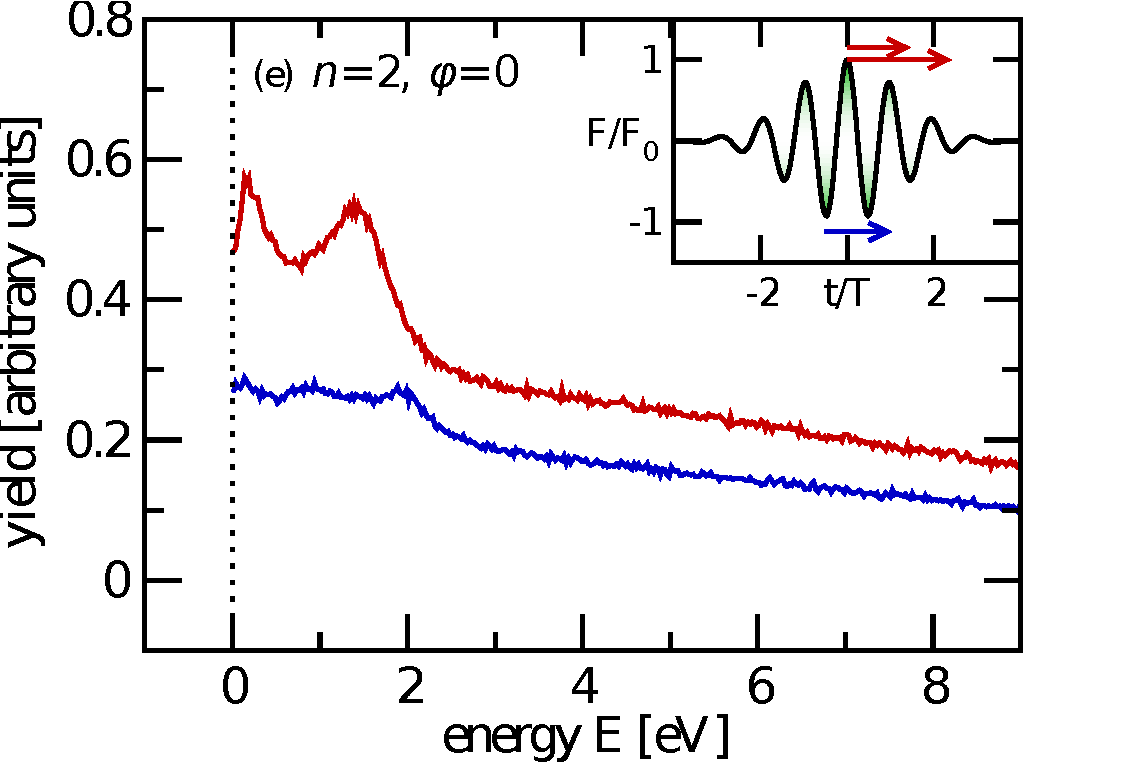
\includegraphics[width=1.2\textwidth, height=201px]{data/kastner.pdf}
 \subcaption{Computed PAD for different energy regions.}
 \label{myPAD} 
\end{subfigure}
\begin{subfigure} [t]{0.5\textwidth}
\hspace{-0.5cm}
  \raisebox{17px}{\resizebox{0.983\textwidth}{!}{\input{data/les.pdf_tex}}}
 \subcaption{Computed ATI spectrum.}
 \label{myATI} 
\end{subfigure}
 \caption{Regions (a), (b) and (c) correspond respectively to $[0, 2U_{p}]$, $[2U_{p}, 8U_{p}]$ and $[8U_{p}, 10U_{p}]$. In right panel, (d) reveals the so-called side lobe which appears for $4U_{p}$}
\end{figure}




\bibliographystyle{unsrt}
\bibliography{mybib}


\end{document}
